\documentclass[letterpaper,10pt,draftclsnofoot,onecolumn,titlepage]{IEEEtran}

\usepackage{graphicx}
\usepackage{amssymb}
\usepackage{amsmath}
\usepackage{amsthm}
\usepackage{alltt}
\usepackage{float}
\usepackage{color}
\usepackage{url}
\usepackage{enumitem}
\usepackage{pstricks, pst-node}
\usepackage{geometry}
\usepackage{array}
\usepackage{listings}
\usepackage{caption}
\usepackage{subcaption}
\usepackage{import}
\usepackage[draft]{pdfpages}


\geometry{margin = .75in}

\usepackage{hyperref}

\usepackage[acronym]{glossaries}

\makeglossaries

\newglossaryentry{iOS}{name={iOS}, description={A mobile operating system created and developed by Apple Inc. exclusively for Apple's hardware}}
\newglossaryentry{ModelVC}{name={Model-View-Controller}, description={A design pattern that assigns objects in an application one of three roles: model, view, or controller. Also called MVC}}
\newglossaryentry{Android}{name={Android}, description={A mobile operating system developed by Google, based on the Linux Kernel and designed primarily for touchscreen mobile devices}}
\newglossaryentry{App}{name={app}, description={A software application designed to run on mobile devices such as smartphones or tablet computers}}
\newacronym{ccb}{CCB}{Church Community Builder}
\newacronym{sdd}{SDD}{Software Design Document}
\newacronym{srs}{SRS}{Software Requirements Specification}
\newacronym{uml}{UML}{Unified Model Language}
\newacronym{mvc}{MVC}{Model-View-Controller}
\newacronym{xml}{XML}{EXtensible Markup Language}
\newacronym{ui}{UI}{User Interface}



\graphicspath{{figures/}{pictures/}{images/}{./}}


\newcommand*{\signature}[1]{%
	\par\noindent\makebox[3.5in]{\hrulefill} \hfill\makebox[3.0in]{\hrulefill}%
	\par\noindent\makebox[3.5in][l]{#1}	    \hfill\makebox[3.0in][l]{Date}%
}%

\def\name{Kevin Stine, Courtney Bonn, Maxwell Dimm}
\def\team{Calvary Chapel Corvallis}
\def\grp{Group \#62}

\hypersetup{
	colorlinks = true,
	urlcolor = black,
	linkcolor = black,
	pdfauthor = {\name},
	pdftitle = {CS463 Final Report},
	pdfsubject = {CS463 Final Report},
	pdfpagemode = UseNone
}

\begin{document}
	\title{\huge \team \\ Final Report\\ CS 463 Spring 2017}
	\author{\large \name \\ \grp}



	\maketitle

		\begin{abstract}The purpose of this project is to produce an iOS/Android application for Calvary Chapel of Corvallis that will allow members to access a plethora of information all in one localized space.
		The Church's current website does not provide an interface where current members of the church can very quickly access important information such as events, bulletins, and messages from the service.
		The desired application will be simple enough for anyone to use while providing back end access for staff to easily upload new information to the app.
		The priorities lie in maximizing the usability of the app and providing bulletin, schedule, video, and giving functionality.
		We will work with the existing Calvary Chapel web development team to create a product that is seamlessly integrated with their already existing network.
		\end{abstract}

		\clearpage
		
		\tableofcontents
		
		\clearpage

\section{Introduction}

\section{Original Requirements}

	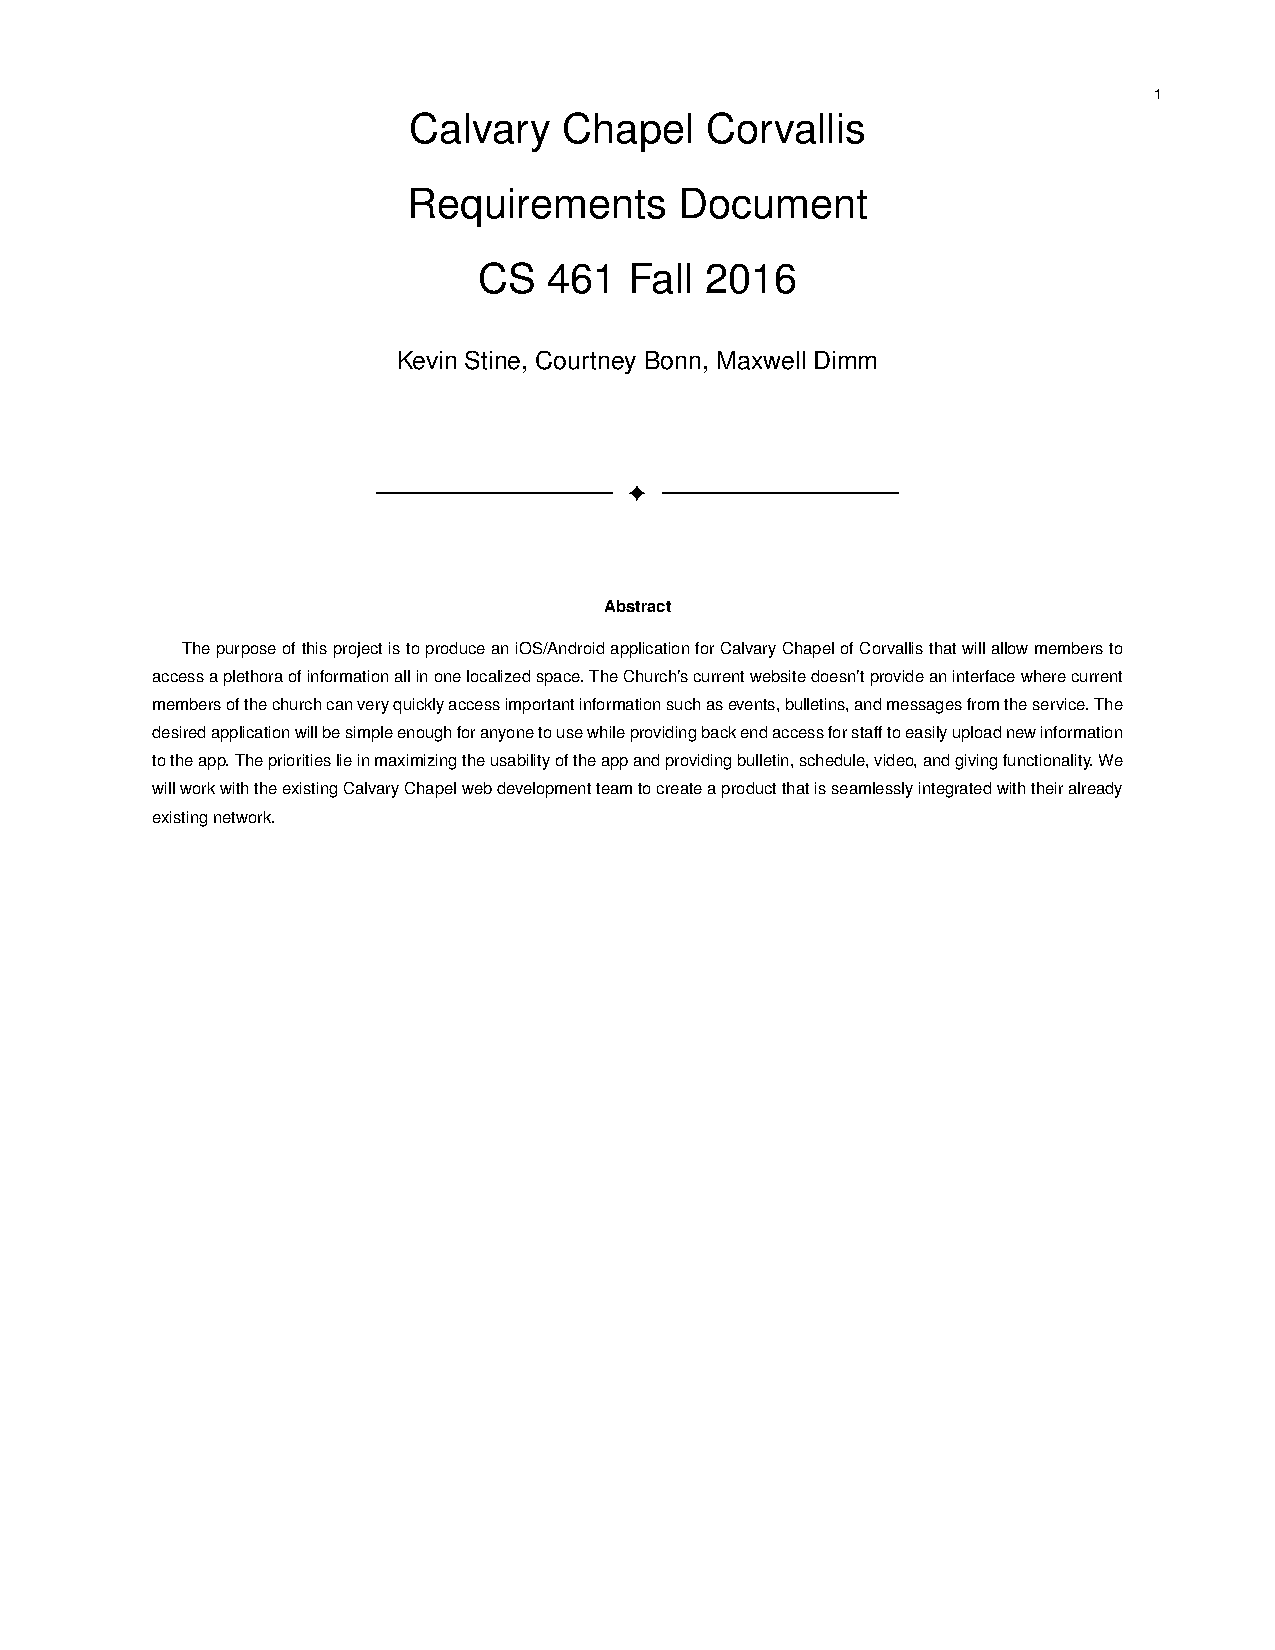
\includepdf[pages={-}]{originals/requirements.pdf}

\section{Requirement Changes}

\section{Original Design Document}

	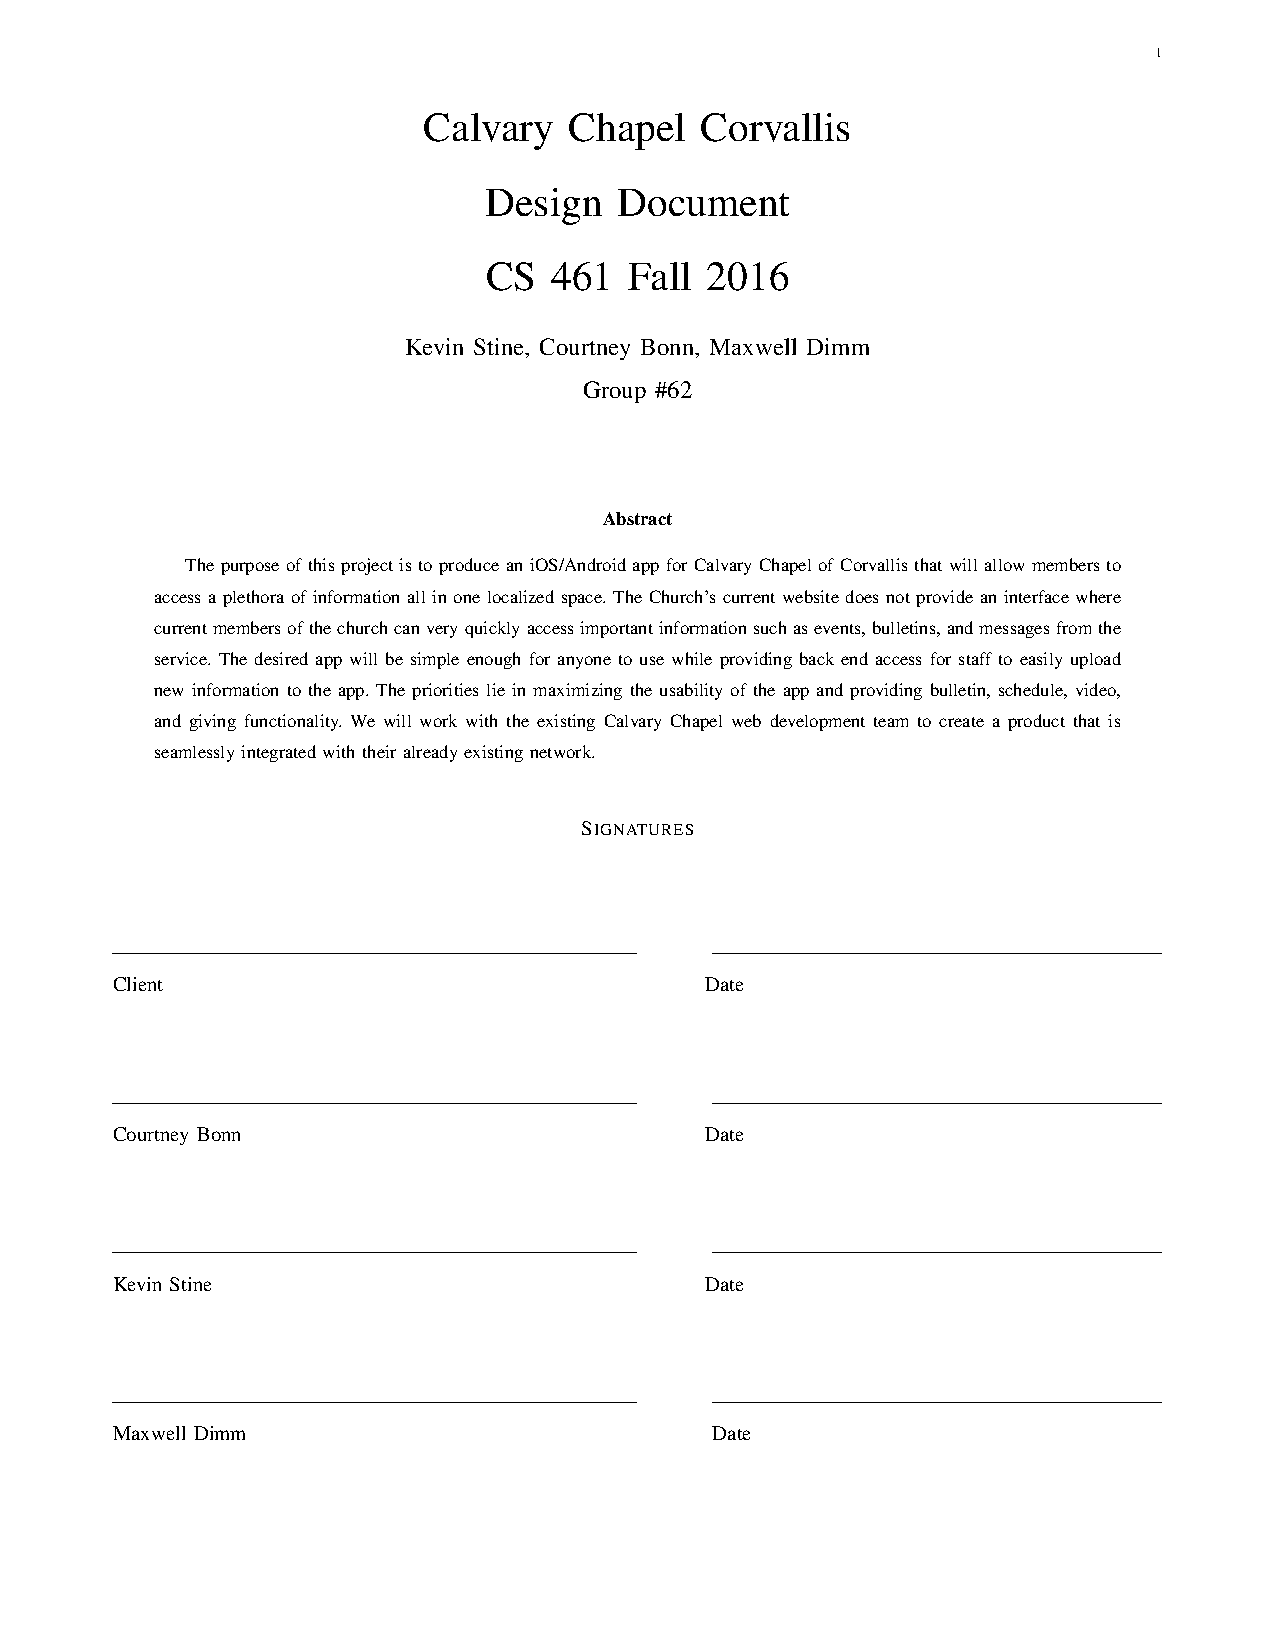
\includepdf[pages={-}]{originals/design.pdf}
	
	\subsection{Design Changes}
	
\section{Original Technology Review}

	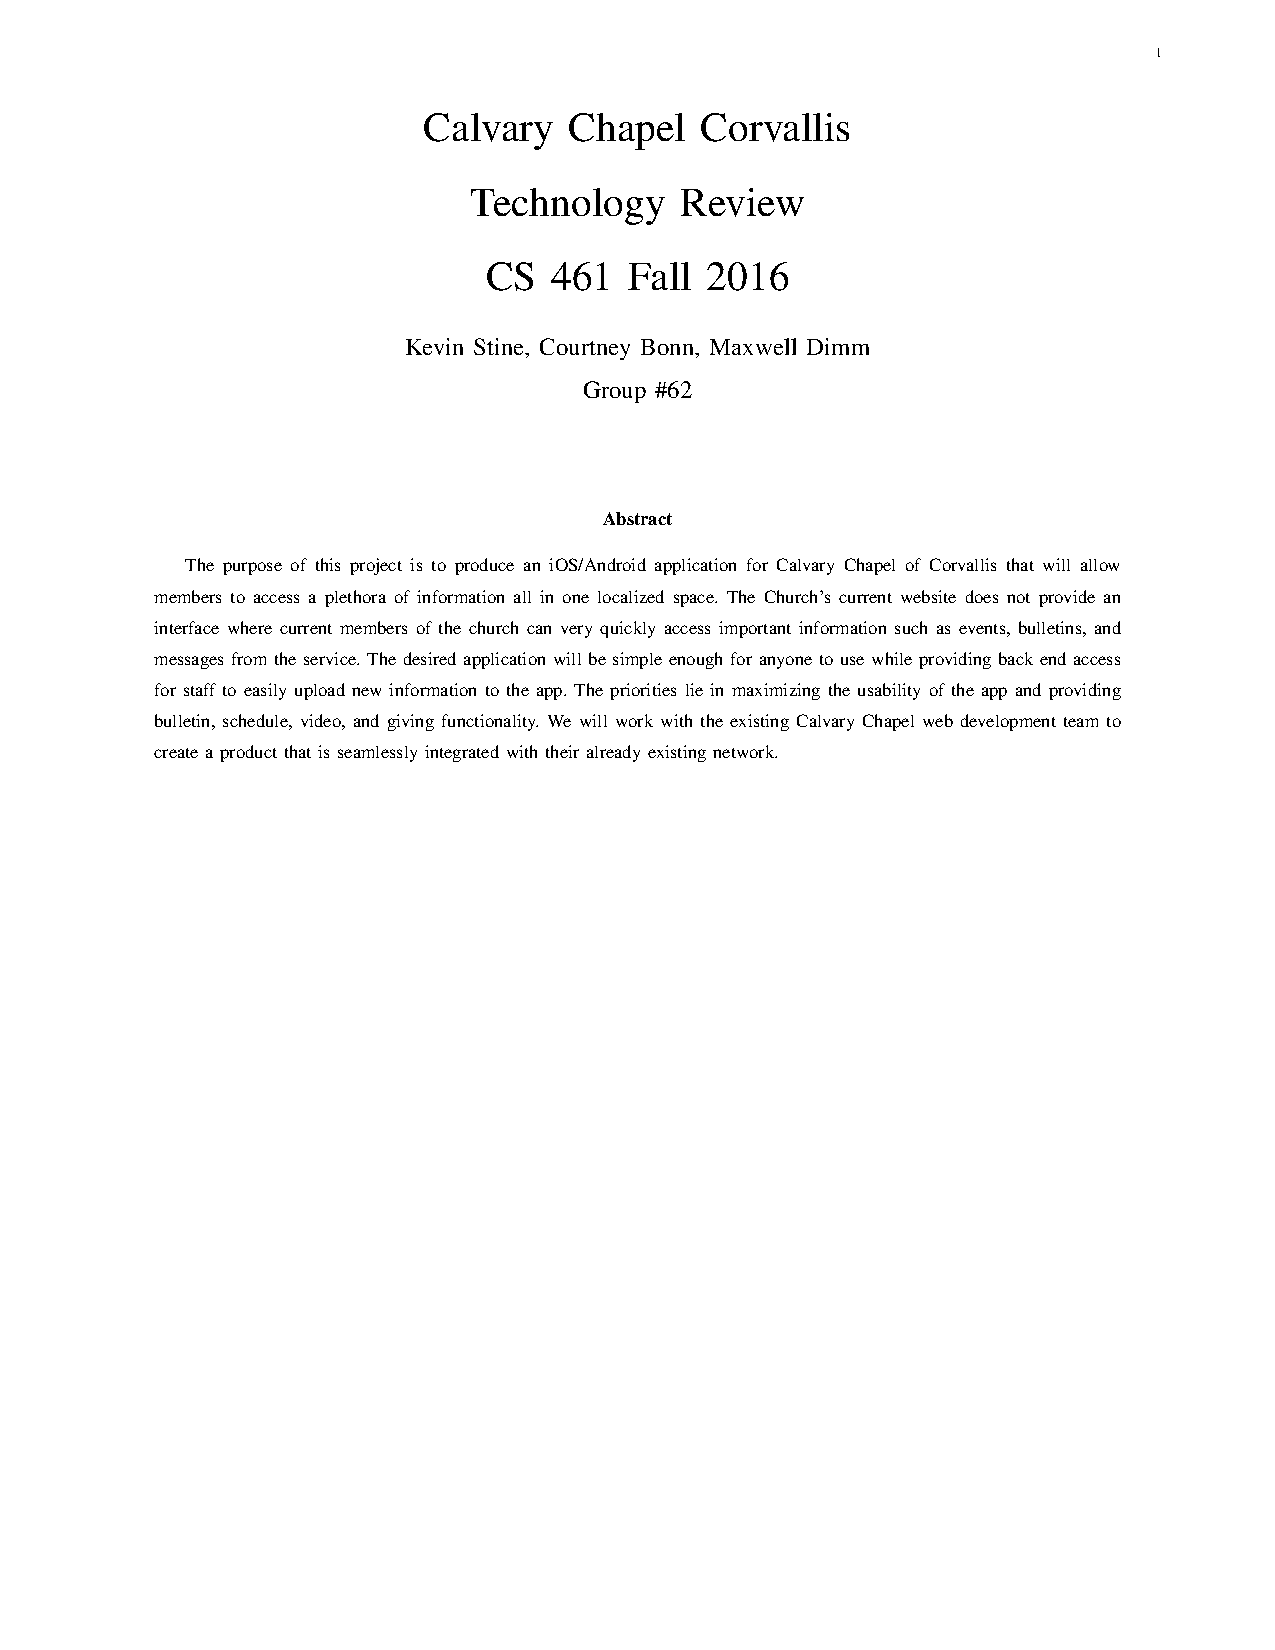
\includepdf[pages={-}]{originals/tech-review.pdf}

	\subsection{Technology Changes}
	
\section{Weekly Blog Posts}

	\import{./}{blogposts}
	
\section{Final Poster}

\section{Project Documentation}

\section{Learning New Technology}

\section{Team Reflection}

	\subsection{Courtney Bonn}
	
	\subsection{Max Dimm}
	
	\subsection{Kevin Stine}
	


\end{document}
